\documentclass[a4paper,12pt]{article}
\usepackage{CJK}
\usepackage{graphicx}
\begin{document}

\begin{CJK}{UTF8}{gkai}
%\begin{CJK}{UTF8}{gbsn}
\section{密码电路故障攻击理论与技术}
\subsection{故障攻击的理论基础:包括攻击原理、基本假设、模型、方法和评价标准。此外,还将阐述一些常用的DFA和其他一些safe error的故障分析方法}
\subsubsection{故障分析的攻击原理和基本攻击方法,包括DFA和IFA,FSA等}

电子设备在运行时会受到各种各样自然的或是人为的干扰,在某些极端条件下设备停止工作或是输出不正确的结果。传统密码分析方法利用密码算法结构和一定明密文对来研究密码安全性,不同与此,故障攻击利用了设备在故障时的不正确结果中隐含的信息来辅助分析。故障攻击主要分为故障注入和故障分析两部分。故障注入主要研究密码设备在受到电压时钟毛刺,激光等干扰时的发生故障的模式;故障分析利用特定的故障输出作为辅助信息来完成密码分析,推导秘密信息。

最早的故障是偶然发生的,放射性元素衰变产生的带电粒子使得芯片出现了故障。之后为了提高芯片的稳定性和可靠性特别当芯片被用于外太空等极端环境下时,研究人员模拟和实验了大量不同的故障环境和对芯片的影响,这阶段研究的主要目的是研制高可靠性设备。

首个利用故障输出来推导密码算法的工作是由*Bellcore*等人在1997年提出的。该方法成功利用一对正确和错误密文对得出使用中国剩余定理实现的RSA算法的私钥。紧随其后故障分析的思想被Biham和Shamir等人用于分组密码DES的分析并提出了对几乎所有分组密码都有效的差分故障攻击。之后研究人员提出了大量的针对各种不同密码算法的故障分析和防护方案,使得故障分析成为一个极为活跃的研究领域。由于故障攻击可以在实际时间内成功攻击密码设备这也导致了对各种专用的故障注入设备的实验和开发。

在现行的软硬件架构和实现中故障注入可以影响程序的执行指令同时也可以影响程序的运算的中间值,对密码算法的故障分析主要集中于影响密码运算中间值的故障类型的分析。影响程序执行指令故障注入可以被用于跳过认证,修改程序流程等多种目的,但是在本章节中我们不考虑这种情况。

\subsubsection{故障模型分类和介绍}

故障模型是对设备在故障注入时产生的影响的抽象描述。故障模型要具有通用性,这样不同的密码算法不同的实现方式都可以通过故障模型加以描述同时这也提供一种便利的叙述背景和比较基准;故障模型也要具有可实现性,故障模型必须是实际的故障注入实验中可以重现的并且这种实现可以基于不同的软硬件设备和不同故障注入手段。

现在的分组密码大部分是迭代式的结构,算法包括多轮大致相同的轮函数,轮函数由几个操作构成,故障注入一般影响某个特定轮的特定操作的中间值或是某几个特定轮中的某个中间值,该中间值的长度一般为分组密码明文长度。在公钥等密码算法中,受影响的中间值一般可以限定为在执行某个操作或是某一组操作时。

一些为大部分研究者所使用和认可的故障模型有单比特故障模型,单字节故障模型。单字节模型,密码算法的中间值的某一比特位的值发生改变,受影响的比特的位置在目标中间值中是随机且均匀分布的,该比特位在受到故障注入影响后随机的变为0或1。单字节故障模型,目标中间值的某一个字节发生改变,受影响的字节的位置在中间值中是随机且均匀分布的,该字节的故障值是随机并且均匀分布的,即故障值为0~255中的任何一个的概率为1/256。

在不同的分析场景下还有一些不同的故障模型,如在safe  error的分析中,一般会假设受影响的比特、字节等的故障值为某一特定值。在轻量级分组密码的分析中,由于它们一般采用比较小(如3X3,4X4)的S盒,研究人员也会采用随机单S盒的故障模型。

随着故障攻击研究的深入,研究人员也在探讨各种新的故障模型,如故障位置或是故障值非均匀分布的故障,多字节的故障模型和更为通用的有偏差非特定型故障模型。

\subsubsection{故障攻击的评价指标,包括所用故障模型,故障数,攻击轮数,攻击的时间复杂度等。}
\subsection{先进分析方法:包括一些当前研究热点,如故障和功耗攻击结合的分析方法}
\subsubsection{故障和传统密码学分析方法的结合}
\subsubsection{故障分析和功耗等旁路分析方法的结合}
\subsubsection{故障攻击在未知但可区分的故障模型下的应用}
\subsection{各类密码结构/算法的故障分析方法:针对常用的对称密码和非对称密码,给出其结构弱点和故障攻击分析方式}
\subsection{DES故障攻击}
1996年,Biham和Shamir第一次提出了对DES的差分故障攻击(DFA),之后又有一些文章对此进行了扩展和改进,本节首先简要介绍DES算法,然后引入针对DES的后两轮原始故障攻击、中间轮故障攻击及基于内部碰撞的前几轮故障攻击。
\subsubsection{DES算法}
DES为64位的16轮Feistel结构(见图\ref{des_feistel}),每一轮的变换为$F_{K_r(L,R)=(R,L \oplus f_{K_r}(R))}$,其中L,R分别表示数据的左右部分,f是以48位密钥$K_r$为参数的32位输入到32位输出的映射函数(见图\ref{des_f_function})
\begin{figure}
\centering
\caption{Des feistel结构}
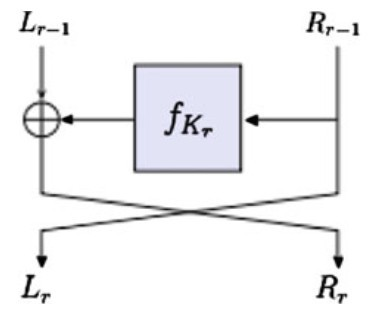
\includegraphics[width=200pt]{Feistel.jpg}
\label{des_feistel}
\end{figure}

\begin{figure}
\centering
\caption{f函数}
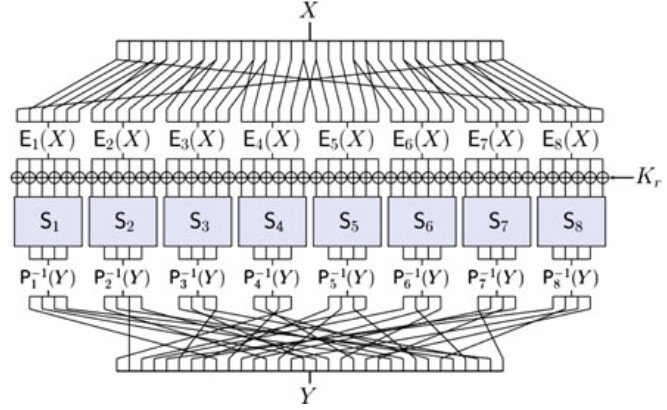
\includegraphics[width=400pt]{des_f_function.jpg}
\label{des_f_function}
\end{figure}


\subsubsection{对DES的第16轮攻击}
假设在第16轮开始的时候,$R_{15}$的一些比特翻转,那么由图\ref{des_feistel}可得$R_{16}$和$R_{16}^*$的差分满足等式:

\begin{equation}
\label{eq:3_1}
\delta R_{16} = f_{K_{16}} \oplus f_{K_{16}}(L_{16}^*)
\end{equation}

由图\ref{des_f_function}可知,f函数中的S盒独立进行计算,所以上式可以转换成8个等式,其中$(1 \leq i \leq 8)$:

\begin{equation}
\label{eq:3_2}
P_i^{-1}(\delta R_{16}) = S_i(E_i(L_{16}) \oplus K_{16,i}) \oplus S_i(E_i(L_{16}^*) \oplus K_{16,i})
\end{equation}

因此攻击者可以通过验证$K_{16,i}$的所有可能值${0,1}^6$,排除不满足等式\ref{eq:3_2}的值,最终得到密钥。值得注意的是本攻击只适用于只影响$R_{15}$的故障故障类型,并且$R_{15}$被故障翻转的比特数越多,有效的S盒也越多(即受影响的S盒),所需要的密文对$(C,C^*)$则越少。

\subsubsection{对DES的第15轮攻击}
假设在第15轮开始的时候,在$R_{14}$上注入单比特故障,令$R_{14}^*=R_{14} \oplus \epsilon$,由图\ref{des_error_propagation_15_round}可得:

\begin{equation}
\label{eq:3_3}
\delta R_{16} = f_{K_{16}}(L_{16}) \oplus f_{K_{16}}(L_{16}^*) \oplus \epsilon
\end{equation}

在上式中$K_{16}$不是唯一的未知参数,因此接下来需要确定或者缩小$\epsilon$的取值范围。利用式\ref{eq:3_4}可以推出第15轮的有效S盒,进而可以根据S盒的有效情况缩小$\epsilon$的取值范围,如果两个S盒有效,则$\epsilon$的值有2种可能,因为由图\ref{des_f_function}可知每对S盒最多共享两个输入比特;同理如果只有一个S盒有效,$\epsilon$的值也有两种可能,因为有效S盒的6个输入比特中与相邻S盒无关的只有2个比特。

\begin{equation}
\label{eq:3_4}
\delta L_{16} = f_{K_{15}}(R_{14}) \oplus f_{K_{15}}(R_{14}) \oplus \epsilon
\end{equation}

\begin{figure}
\centering
\caption{15轮的错误扩散}
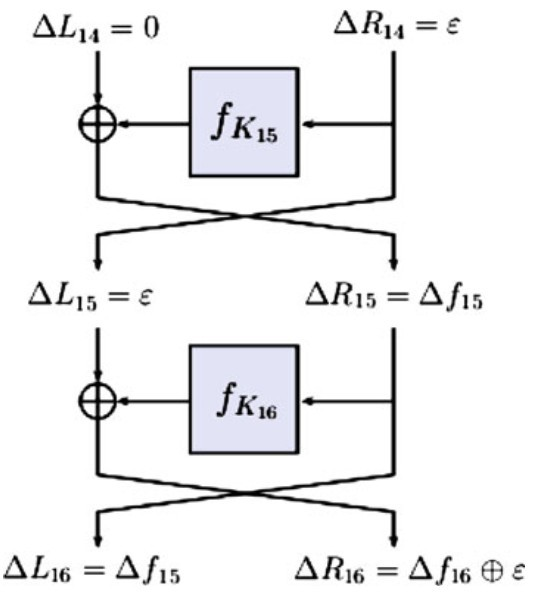
\includegraphics[width=200pt]{des_15_round_propagation.jpg}
\label{des_error_propagation_15_round}
\end{figure}

一旦$\epsilon$的范围确定,就可以用等式\ref{eq:3_3}推出8等式\ref{eq:3_5}(其中$1 \leq i \leq 8$),进而筛选出密钥$K_{16}$。

\begin{equation}
\label{eq:3_5}
P_i^{-1}(\delta R_{16} \oplus \epsilon) = S_i(E_i(L_{16}) \oplus K_{16,i}) \oplus S_i(E_i(L_{16}^*) \oplus K_{16,i})
\end{equation}

与上一节的攻击相比,本攻击为单比特故障模型(或者只有很少的几个比特故障),因为需要缩小$\epsilon$的取值范围。又因为在第16轮错误被扩散到多个S盒,所以$K_{16}$的筛选效率并不比第16轮的攻击低多少。

\subsubsection{AES故障攻击}

自从2000年被选为Advanced Encryption Standard(AES),Rijndael得到了越来越多的应用,出现了大量关于AES故障攻击的研究。本节选取几种最为典型的针对AES的故障攻击加以描述。

128比特密钥和192,256比特密钥

下面描述的第一种攻击采用随机单字节故障模型,故障注入在倒数第二轮且在列置换操作之前的任一字节。此时攻击的目标状态为倒数第二轮的列置换之前,经过一轮的故障传播在该目标状态的每一列有且仅有一个字节的正确错误状态的差分值非零。攻击者猜测最后一轮子密钥的四字节,对正确和错误密文分别进行部分解密,根据目标状态相应列是否符合前句所述的模式即可排除错误的密钥的猜测。每组这样的猜测可以用于确定相关四字节的子密钥,因此通过四组这样的猜测就可以最后一轮子密钥的恢复。已有的模拟实验显示通过2组正确错误密文对攻击者能以92%的概率唯一的确定最后一轮的轮密钥。

上述攻击的故障模型比较简洁,第二种攻击采用更为复杂的故障模型。可以观察到,当故障发生在倒数第三轮的输入状态的某一对角线时,本轮结束时的状态的差分值全部集中在一列上。在倒数第二轮的列置换之前每一列仍然只有一个字节的差分值不为0.若故障注入在第一对角线,经过推导可以的得出如下等式。

	\begin{equation}

	SB^{-1}(C_{0}\oplus K^{r}_{0}) \oplus SB^{-1}(C'_{0} \oplus K^{r}_{0} ) = 2(SB^{-1}(C_{13}\oplus K^{r}_{13}) \oplus SB^{-1}(C'_{13} \oplus K^{r}_{13} ) )

	SB^{-1}(C_{10}\oplus K^{r}_{10}) \oplus SB^{-1}(C'_{10} \oplus K^{r}_{10} ) = SB^{-1}(C_{13}\oplus K^{r}_{13}) \oplus SB^{-1}(C'_{13} \oplus K^{r}_{13} )

	SB^{-1}(C_{7}\oplus K^{r}_{7}) \oplus SB^{-1}(C'_{7} \oplus K^{r}_{7} ) = 3(SB^{-1}(C_{13}\oplus K^{r}_{13}) \oplus SB^{-1}(C'_{13} \oplus K^{r}_{13} ) )
	\end{equation}
攻击者首先猜测$K^{r}_{0}$和$K^{r}_{13}$,如果猜测值满足上述第一个等式则保留为候选密钥字节,否则为错误密钥。结合$K^{r}_{13}$的候选值和$K^{r}_{10}$的所有可能值并测试其是否满足上述第二个等式可以进一步减少密钥空间,随后将同样的方法运用到第三个等式,通过以上三组操作$(K^{r}_{0}, K^{r}_{7}, K^{r}_{10}, K^{r}_{13})$的可能值的数量平均为$2^{8} = 256$个。

对于目标状态的其他三列也有类似的结果,这样最后可以将最后一轮轮密钥的密钥空间降低到$(2^{8})^{4}=2^{32}$。上述讨论中故障所处的对角线已知,如果故障发生的对角线未知,需要猜测所有可能四种情况,密钥空间是已知对角线情况的4倍。

上述攻击可以被扩展到在倒数第三轮的输入状态上至多三个对角线上的值受影响的故障模型。此时可以列出类似上述所示等式组,具体的等式会稍微比较复杂,如果没有发生故障的对角线已知,等式组成的密钥区分器可以将猜测的4字节的密钥空间降低到$2^{24}$。在这样的故障模型下,使用四对正确错误密文对,最后一轮轮密钥可以以很大的概率确定。

\subsubsection{RSA故障攻击}
\subsubsection{ECC故障攻击}
\subsubsection{其他算法包括轻量级算法的故障分析}
\subsubsection{流密码和哈希函数的故障攻击简介}
\subsection{故障攻击实验环境:包括已有的故障攻击实施工具和攻击过程,如电压和时钟Glitch,激光和电磁辐射等}
\subsubsection{电压和时钟的故障实验环境和注入结果}
\subsubsection{电磁辐射的故障实验环境和注入结果}
\subsubsection{激光的故障实验环境和注入结果}
\subsubsection{多点故障注入的实验环境和实验结果}
\subsubsection{抗故障攻击的防御方法:已有的抗故障攻击防御技术}
\subsubsection{冗余计算的防护方案}
\subsubsection{掩码防护方案}
\subsubsection{抗故障攻击的电路单元}
\end{CJK}


\end{document}